\documentclass[1p]{elsarticle_modified}
%\bibliographystyle{elsarticle-num}

%\usepackage[colorlinks]{hyperref}
%\usepackage{abbrmath_seonhwa} %\Abb, \Ascr, \Acal ,\Abf, \Afrak
\usepackage{amsfonts}
\usepackage{amssymb}
\usepackage{amsmath}
\usepackage{amsthm}
\usepackage{scalefnt}
\usepackage{amsbsy}
\usepackage{kotex}
\usepackage{caption}
\usepackage{subfig}
\usepackage{color}
\usepackage{graphicx}
\usepackage{xcolor} %% white, black, red, green, blue, cyan, magenta, yellow
\usepackage{float}
\usepackage{setspace}
\usepackage{hyperref}

\usepackage{tikz}
\usetikzlibrary{arrows}

\usepackage{multirow}
\usepackage{array} % fixed length table
\usepackage{hhline}

%%%%%%%%%%%%%%%%%%%%%
\makeatletter
\renewcommand*\env@matrix[1][\arraystretch]{%
	\edef\arraystretch{#1}%
	\hskip -\arraycolsep
	\let\@ifnextchar\new@ifnextchar
	\array{*\c@MaxMatrixCols c}}
\makeatother %https://tex.stackexchange.com/questions/14071/how-can-i-increase-the-line-spacing-in-a-matrix
%%%%%%%%%%%%%%%

\usepackage[normalem]{ulem}

\newcommand{\msout}[1]{\ifmmode\text{\sout{\ensuremath{#1}}}\else\sout{#1}\fi}
%SOURCE: \msout is \stkout macro in https://tex.stackexchange.com/questions/20609/strikeout-in-math-mode

\newcommand{\cancel}[1]{
	\ifmmode
	{\color{red}\msout{#1}}
	\else
	{\color{red}\sout{#1}}
	\fi
}

\newcommand{\add}[1]{
	{\color{blue}\uwave{#1}}
}

\newcommand{\replace}[2]{
	\ifmmode
	{\color{red}\msout{#1}}{\color{blue}\uwave{#2}}
	\else
	{\color{red}\sout{#1}}{\color{blue}\uwave{#2}}
	\fi
}

\newcommand{\Sol}{\mathcal{S}} %segment
\newcommand{\D}{D} %diagram
\newcommand{\A}{\mathcal{A}} %arc


%%%%%%%%%%%%%%%%%%%%%%%%%%%%%5 test

\def\sl{\operatorname{\textup{SL}}(2,\Cbb)}
\def\psl{\operatorname{\textup{PSL}}(2,\Cbb)}
\def\quan{\mkern 1mu \triangleright \mkern 1mu}

\theoremstyle{definition}
\newtheorem{thm}{Theorem}[section]
\newtheorem{prop}[thm]{Proposition}
\newtheorem{lem}[thm]{Lemma}
\newtheorem{ques}[thm]{Question}
\newtheorem{cor}[thm]{Corollary}
\newtheorem{defn}[thm]{Definition}
\newtheorem{exam}[thm]{Example}
\newtheorem{rmk}[thm]{Remark}
\newtheorem{alg}[thm]{Algorithm}

\newcommand{\I}{\sqrt{-1}}
\begin{document}

%\begin{frontmatter}
%
%\title{Boundary parabolic representations of knots up to 8 crossings}
%
%%% Group authors per affiliation:
%\author{Yunhi Cho} 
%\address{Department of Mathematics, University of Seoul, Seoul, Korea}
%\ead{yhcho@uos.ac.kr}
%
%
%\author{Seonhwa Kim} %\fnref{s_kim}}
%\address{Center for Geometry and Physics, Institute for Basic Science, Pohang, 37673, Korea}
%\ead{ryeona17@ibs.re.kr}
%
%\author{Hyuk Kim}
%\address{Department of Mathematical Sciences, Seoul National University, Seoul 08826, Korea}
%\ead{hyukkim@snu.ac.kr}
%
%\author{Seokbeom Yoon}
%\address{Department of Mathematical Sciences, Seoul National University, Seoul, 08826,  Korea}
%\ead{sbyoon15@snu.ac.kr}
%
%\begin{abstract}
%We find all boundary parabolic representation of knots up to 8 crossings.
%
%\end{abstract}
%\begin{keyword}
%    \MSC[2010] 57M25 
%\end{keyword}
%
%\end{frontmatter}

%\linenumbers
%\tableofcontents
%
\newcommand\colored[1]{\textcolor{white}{\rule[-0.35ex]{0.8em}{1.4ex}}\kern-0.8em\color{red} #1}%
%\newcommand\colored[1]{\textcolor{white}{ #1}\kern-2.17ex	\textcolor{white}{ #1}\kern-1.81ex	\textcolor{white}{ #1}\kern-2.15ex\color{red}#1	}

{\Large $\underline{12n_{0867}~(K12n_{0867})}$}

\setlength{\tabcolsep}{10pt}
\renewcommand{\arraystretch}{1.6}
\vspace{1cm}\begin{tabular}{m{100pt}>{\centering\arraybackslash}m{274pt}}
\multirow{5}{120pt}{
	\centering
	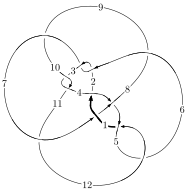
\includegraphics[width=112pt]{../../../GIT/diagram.site/Diagrams/png/2956_12n_0867.png}\\
\ \ \ A knot diagram\footnotemark}&
\allowdisplaybreaks
\textbf{Linearized knot diagam} \\
\cline{2-2}
 &
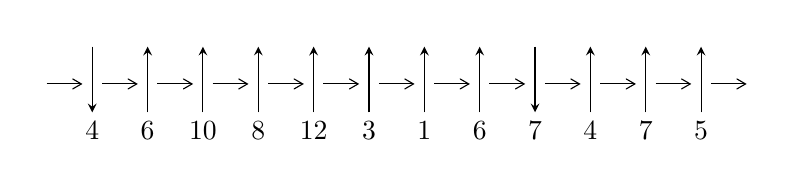
\begin{tikzpicture}[x=20pt, y=17pt]
	% nodes
	\node (C0) at (0, 0) {};
	\node (C1) at (1, 0) {};
	\node (C1U) at (1, +1) {};
	\node (C1D) at (1, -1) {4};

	\node (C2) at (2, 0) {};
	\node (C2U) at (2, +1) {};
	\node (C2D) at (2, -1) {6};

	\node (C3) at (3, 0) {};
	\node (C3U) at (3, +1) {};
	\node (C3D) at (3, -1) {10};

	\node (C4) at (4, 0) {};
	\node (C4U) at (4, +1) {};
	\node (C4D) at (4, -1) {8};

	\node (C5) at (5, 0) {};
	\node (C5U) at (5, +1) {};
	\node (C5D) at (5, -1) {12};

	\node (C6) at (6, 0) {};
	\node (C6U) at (6, +1) {};
	\node (C6D) at (6, -1) {3};

	\node (C7) at (7, 0) {};
	\node (C7U) at (7, +1) {};
	\node (C7D) at (7, -1) {1};

	\node (C8) at (8, 0) {};
	\node (C8U) at (8, +1) {};
	\node (C8D) at (8, -1) {6};

	\node (C9) at (9, 0) {};
	\node (C9U) at (9, +1) {};
	\node (C9D) at (9, -1) {7};

	\node (C10) at (10, 0) {};
	\node (C10U) at (10, +1) {};
	\node (C10D) at (10, -1) {4};

	\node (C11) at (11, 0) {};
	\node (C11U) at (11, +1) {};
	\node (C11D) at (11, -1) {7};

	\node (C12) at (12, 0) {};
	\node (C12U) at (12, +1) {};
	\node (C12D) at (12, -1) {5};
	\node (C13) at (13, 0) {};

	% arrows
	\draw[->,>={angle 60}]
	(C0) edge (C1) (C1) edge (C2) (C2) edge (C3) (C3) edge (C4) (C4) edge (C5) (C5) edge (C6) (C6) edge (C7) (C7) edge (C8) (C8) edge (C9) (C9) edge (C10) (C10) edge (C11) (C11) edge (C12) (C12) edge (C13) ;	\draw[->,>=stealth]
	(C1U) edge (C1D) (C2D) edge (C2U) (C3D) edge (C3U) (C4D) edge (C4U) (C5D) edge (C5U) (C6D) edge (C6U) (C7D) edge (C7U) (C8D) edge (C8U) (C9U) edge (C9D) (C10D) edge (C10U) (C11D) edge (C11U) (C12D) edge (C12U) ;
	\end{tikzpicture} \\
\hhline{~~} \\& 
\textbf{Solving Sequence} \\ \cline{2-2} 
 &
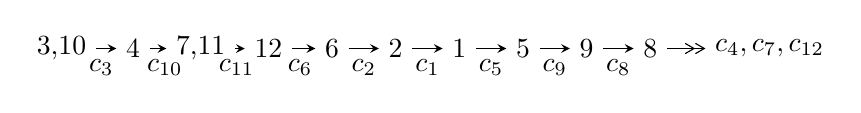
\begin{tikzpicture}[x=23pt, y=7pt]
	% node
	\node (A0) at (-1/8, 0) {3,10};
	\node (A1) at (1, 0) {4};
	\node (A2) at (33/16, 0) {7,11};
	\node (A3) at (25/8, 0) {12};
	\node (A4) at (33/8, 0) {6};
	\node (A5) at (41/8, 0) {2};
	\node (A6) at (49/8, 0) {1};
	\node (A7) at (57/8, 0) {5};
	\node (A8) at (65/8, 0) {9};
	\node (A9) at (73/8, 0) {8};
	\node (C1) at (1/2, -1) {$c_{3}$};
	\node (C2) at (3/2, -1) {$c_{10}$};
	\node (C3) at (21/8, -1) {$c_{11}$};
	\node (C4) at (29/8, -1) {$c_{6}$};
	\node (C5) at (37/8, -1) {$c_{2}$};
	\node (C6) at (45/8, -1) {$c_{1}$};
	\node (C7) at (53/8, -1) {$c_{5}$};
	\node (C8) at (61/8, -1) {$c_{9}$};
	\node (C9) at (69/8, -1) {$c_{8}$};
	\node (A10) at (11, 0) {$c_{4},c_{7},c_{12}$};

	% edge
	\draw[->,>=stealth]	
	(A0) edge (A1) (A1) edge (A2) (A2) edge (A3) (A3) edge (A4) (A4) edge (A5) (A5) edge (A6) (A6) edge (A7) (A7) edge (A8) (A8) edge (A9) ;
	\draw[->>,>={angle 60}]	
	(A9) edge (A10);
\end{tikzpicture} \\ 

\end{tabular} \\

\footnotetext{
The image of knot diagram is generated by the software ``\textbf{Draw programme}" developed by Andrew Bartholomew(\url{http://www.layer8.co.uk/maths/draw/index.htm\#Running-draw}), where we modified some parts for our purpose(\url{https://github.com/CATsTAILs/LinksPainter}).
}\phantom \\ \newline 
\centering \textbf{Ideals for irreducible components\footnotemark of $X_{\text{par}}$} 
 
\begin{align*}
I^u_{1}&=\langle 
b- u,\;-81072715476 u^{25}+52576364860 u^{24}+\cdots+3386368973 a+151407587225,\\
\phantom{I^u_{1}}&\phantom{= \langle  }u^{26}-7 u^{24}+\cdots-2 u-1\rangle \\
I^u_{2}&=\langle 
-6.03995\times10^{146} u^{63}-9.04955\times10^{146} u^{62}+\cdots+5.66297\times10^{148} b-4.48747\times10^{149},\\
\phantom{I^u_{2}}&\phantom{= \langle  }-1.13952\times10^{150} u^{63}-1.92915\times10^{150} u^{62}+\cdots+4.19060\times10^{150} a-1.96444\times10^{152},\\
\phantom{I^u_{2}}&\phantom{= \langle  }u^{64}+2 u^{63}+\cdots+171 u+37\rangle \\
I^u_{3}&=\langle 
b+u,\;106 u^{13}-38 u^{12}+\cdots+29 a+111,\;u^{14}-4 u^{12}+8 u^{10}-10 u^8+u^7+5 u^6- u^5+2 u^4- u^3-2 u^2+u+1\rangle \\
I^u_{4}&=\langle 
u^{11}-4 u^9+5 u^7-3 u^5+5 u^3+b-4 u,\\
\phantom{I^u_{4}}&\phantom{= \langle  }-3 u^{11}-4 u^{10}+11 u^9+14 u^8-11 u^7-13 u^6+4 u^5+5 u^4-12 u^3-17 u^2+2 a+8 u+8,\\
\phantom{I^u_{4}}&\phantom{= \langle  }u^{12}-4 u^{10}+5 u^8-3 u^6+5 u^4-4 u^2+1\rangle \\
I^u_{5}&=\langle 
b+u-1,\;a+u-1,\;u^2- u+1\rangle \\
\\
\end{align*}
\raggedright * 5 irreducible components of $\dim_{\mathbb{C}}=0$, with total 118 representations.\\
\footnotetext{All coefficients of polynomials are rational numbers. But the coefficients are sometimes approximated in decimal forms when there is not enough margin.}
\newpage
\renewcommand{\arraystretch}{1}
\centering \section*{I. $I^u_{1}= \langle b- u,\;-8.11\times10^{10} u^{25}+5.26\times10^{10} u^{24}+\cdots+3.39\times10^{9} a+1.51\times10^{11},\;u^{26}-7 u^{24}+\cdots-2 u-1 \rangle$}
\flushleft \textbf{(i) Arc colorings}\\
\begin{tabular}{m{7pt} m{180pt} m{7pt} m{180pt} }
\flushright $a_{3}=$&$\begin{pmatrix}1\\0\end{pmatrix}$ \\
\flushright $a_{10}=$&$\begin{pmatrix}0\\u\end{pmatrix}$ \\
\flushright $a_{4}=$&$\begin{pmatrix}1\\- u^2\end{pmatrix}$ \\
\flushright $a_{7}=$&$\begin{pmatrix}23.9409 u^{25}-15.5259 u^{24}+\cdots-17.7599 u-44.7109\\u\end{pmatrix}$ \\
\flushright $a_{11}=$&$\begin{pmatrix}u\\- u^3+u\end{pmatrix}$ \\
\flushright $a_{12}=$&$\begin{pmatrix}14.9186 u^{25}-4.47512 u^{24}+\cdots+9.17407 u-31.5817\\5.21774 u^{25}-3.42933 u^{24}+\cdots-2.57347 u-10.1364\end{pmatrix}$ \\
\flushright $a_{6}=$&$\begin{pmatrix}23.9409 u^{25}-15.5259 u^{24}+\cdots-18.7599 u-44.7109\\u\end{pmatrix}$ \\
\flushright $a_{2}=$&$\begin{pmatrix}-15.5259 u^{25}+7.24164 u^{24}+\cdots+3.17090 u+24.9409\\u^2\end{pmatrix}$ \\
\flushright $a_{1}=$&$\begin{pmatrix}-20.9154 u^{25}+9.26554 u^{24}+\cdots+2.12830 u+32.1825\\1.96019 u^{25}-0.497707 u^{24}+\cdots+1.34172 u-2.02390\end{pmatrix}$ \\
\flushright $a_{5}=$&$\begin{pmatrix}-46.2583 u^{25}+23.0203 u^{24}+\cdots+7.38663 u+78.1426\\2.51848 u^{25}-0.734211 u^{24}+\cdots+3.08951 u-4.29711\end{pmatrix}$ \\
\flushright $a_{9}=$&$\begin{pmatrix}27.4397 u^{25}-10.7838 u^{24}+\cdots+6.93525 u-57.8914\\7.24164 u^{25}-5.38952 u^{24}+\cdots-6.11087 u-15.5259\end{pmatrix}$ \\
\flushright $a_{8}=$&$\begin{pmatrix}17.7388 u^{25}-9.73803 u^{24}+\cdots-4.81229 u-36.4461\\2.02390 u^{25}-1.96019 u^{24}+\cdots-2.53740 u-5.38952\end{pmatrix}$\\&\end{tabular}
\flushleft \textbf{(ii) Obstruction class $= -1$}\\~\\
\flushleft \textbf{(iii) Cusp Shapes $= \frac{39142336274}{3386368973} u^{25}-\frac{35272648620}{3386368973} u^{24}+\cdots-\frac{7281974472}{260489921} u-\frac{23728803050}{3386368973}$}\\~\\
\newpage\renewcommand{\arraystretch}{1}
\flushleft \textbf{(iv) u-Polynomials at the component}\newline \\
\begin{tabular}{m{50pt}|m{274pt}}
Crossings & \hspace{64pt}u-Polynomials at each crossing \\
\hline $$\begin{aligned}c_{1}\end{aligned}$$&$\begin{aligned}
&u^{26}-21 u^{25}+\cdots+7680 u-512
\end{aligned}$\\
\hline $$\begin{aligned}c_{2},c_{3},c_{6}\\c_{10}\end{aligned}$$&$\begin{aligned}
&u^{26}-7 u^{24}+\cdots+2 u-1
\end{aligned}$\\
\hline $$\begin{aligned}c_{4},c_{7}\end{aligned}$$&$\begin{aligned}
&u^{26}+5 u^{24}+\cdots-8 u+1
\end{aligned}$\\
\hline $$\begin{aligned}c_{5},c_{12}\end{aligned}$$&$\begin{aligned}
&u^{26}-11 u^{25}+\cdots+304 u-24
\end{aligned}$\\
\hline $$\begin{aligned}c_{8},c_{11}\end{aligned}$$&$\begin{aligned}
&u^{26}-2 u^{25}+\cdots-80 u+19
\end{aligned}$\\
\hline $$\begin{aligned}c_{9}\end{aligned}$$&$\begin{aligned}
&u^{26}-21 u^{25}+\cdots-16284 u+1096
\end{aligned}$\\
\hline
\end{tabular}\\~\\
\newpage\renewcommand{\arraystretch}{1}
\flushleft \textbf{(v) Riley Polynomials at the component}\newline \\
\begin{tabular}{m{50pt}|m{274pt}}
Crossings & \hspace{64pt}Riley Polynomials at each crossing \\
\hline $$\begin{aligned}c_{1}\end{aligned}$$&$\begin{aligned}
&y^{26}- y^{25}+\cdots-3932160 y+262144
\end{aligned}$\\
\hline $$\begin{aligned}c_{2},c_{3},c_{6}\\c_{10}\end{aligned}$$&$\begin{aligned}
&y^{26}-14 y^{25}+\cdots-24 y+1
\end{aligned}$\\
\hline $$\begin{aligned}c_{4},c_{7}\end{aligned}$$&$\begin{aligned}
&y^{26}+10 y^{25}+\cdots-36 y+1
\end{aligned}$\\
\hline $$\begin{aligned}c_{5},c_{12}\end{aligned}$$&$\begin{aligned}
&y^{26}+17 y^{25}+\cdots-2656 y+576
\end{aligned}$\\
\hline $$\begin{aligned}c_{8},c_{11}\end{aligned}$$&$\begin{aligned}
&y^{26}+22 y^{25}+\cdots-7236 y+361
\end{aligned}$\\
\hline $$\begin{aligned}c_{9}\end{aligned}$$&$\begin{aligned}
&y^{26}+5 y^{25}+\cdots-35876688 y+1201216
\end{aligned}$\\
\hline
\end{tabular}\\~\\
\newpage\flushleft \textbf{(vi) Complex Volumes and Cusp Shapes}
$$\begin{array}{c|c|c}  
\text{Solutions to }I^u_{1}& \I (\text{vol} + \sqrt{-1}CS) & \text{Cusp shape}\\
 \hline 
\begin{aligned}
u &= -0.783583 + 0.497565 I \\
a &= -0.552401 + 0.963003 I \\
b &= -0.783583 + 0.497565 I\end{aligned}
 & \phantom{-}2.97189 - 1.12917 I & \phantom{-}11.90635 + 3.31876 I \\ \hline\begin{aligned}
u &= -0.783583 - 0.497565 I \\
a &= -0.552401 - 0.963003 I \\
b &= -0.783583 - 0.497565 I\end{aligned}
 & \phantom{-}2.97189 + 1.12917 I & \phantom{-}11.90635 - 3.31876 I \\ \hline\begin{aligned}
u &= -1.086820 + 0.182504 I \\
a &= \phantom{-}0.465254 - 0.140063 I \\
b &= -1.086820 + 0.182504 I\end{aligned}
 & \phantom{-}1.13119 - 2.61384 I & \phantom{-}9.69860 + 3.81800 I \\ \hline\begin{aligned}
u &= -1.086820 - 0.182504 I \\
a &= \phantom{-}0.465254 + 0.140063 I \\
b &= -1.086820 - 0.182504 I\end{aligned}
 & \phantom{-}1.13119 + 2.61384 I & \phantom{-}9.69860 - 3.81800 I \\ \hline\begin{aligned}
u &= \phantom{-}1.086220 + 0.199675 I \\
a &= \phantom{-}0.091019 + 0.925043 I \\
b &= \phantom{-}1.086220 + 0.199675 I\end{aligned}
 & \phantom{-}2.34848 - 2.40757 I & \phantom{-}11.72048 + 1.43873 I \\ \hline\begin{aligned}
u &= \phantom{-}1.086220 - 0.199675 I \\
a &= \phantom{-}0.091019 - 0.925043 I \\
b &= \phantom{-}1.086220 - 0.199675 I\end{aligned}
 & \phantom{-}2.34848 + 2.40757 I & \phantom{-}11.72048 - 1.43873 I \\ \hline\begin{aligned}
u &= \phantom{-}0.793430 + 0.080832 I \\
a &= -0.31402 + 1.95659 I \\
b &= \phantom{-}0.793430 + 0.080832 I\end{aligned}
 & \phantom{-}2.86846 - 2.53404 I & \phantom{-}13.29449 + 3.41848 I \\ \hline\begin{aligned}
u &= \phantom{-}0.793430 - 0.080832 I \\
a &= -0.31402 - 1.95659 I \\
b &= \phantom{-}0.793430 - 0.080832 I\end{aligned}
 & \phantom{-}2.86846 + 2.53404 I & \phantom{-}13.29449 - 3.41848 I \\ \hline\begin{aligned}
u &= \phantom{-}0.843436 + 0.905238 I \\
a &= -0.58396 + 1.35722 I \\
b &= \phantom{-}0.843436 + 0.905238 I\end{aligned}
 & -8.06090 - 4.16985 I & \phantom{-}4.50695 + 1.21035 I \\ \hline\begin{aligned}
u &= \phantom{-}0.843436 - 0.905238 I \\
a &= -0.58396 - 1.35722 I \\
b &= \phantom{-}0.843436 - 0.905238 I\end{aligned}
 & -8.06090 + 4.16985 I & \phantom{-}4.50695 - 1.21035 I\\
 \hline 
 \end{array}$$\newpage$$\begin{array}{c|c|c}  
\text{Solutions to }I^u_{1}& \I (\text{vol} + \sqrt{-1}CS) & \text{Cusp shape}\\
 \hline 
\begin{aligned}
u &= \phantom{-}1.27855\phantom{ +0.000000I} \\
a &= -1.03578\phantom{ +0.000000I} \\
b &= \phantom{-}1.27855\phantom{ +0.000000I}\end{aligned}
 & \phantom{-}6.69425\phantom{ +0.000000I} & -5.31560\phantom{ +0.000000I} \\ \hline\begin{aligned}
u &= -0.947242 + 0.861971 I \\
a &= \phantom{-}0.449801 + 1.090630 I \\
b &= -0.947242 + 0.861971 I\end{aligned}
 & -2.70506 - 1.24876 I & \phantom{-}6.24886 - 0.86995 I \\ \hline\begin{aligned}
u &= -0.947242 - 0.861971 I \\
a &= \phantom{-}0.449801 - 1.090630 I \\
b &= -0.947242 - 0.861971 I\end{aligned}
 & -2.70506 + 1.24876 I & \phantom{-}6.24886 + 0.86995 I \\ \hline\begin{aligned}
u &= -1.152600 + 0.696627 I \\
a &= \phantom{-}0.876822 + 1.038740 I \\
b &= -1.152600 + 0.696627 I\end{aligned}
 & -4.95525 - 4.75697 I & \phantom{-}1.31627 + 5.46968 I \\ \hline\begin{aligned}
u &= -1.152600 - 0.696627 I \\
a &= \phantom{-}0.876822 - 1.038740 I \\
b &= -1.152600 - 0.696627 I\end{aligned}
 & -4.95525 + 4.75697 I & \phantom{-}1.31627 - 5.46968 I \\ \hline\begin{aligned}
u &= \phantom{-}0.983614 + 0.927361 I \\
a &= -0.149538 + 1.130440 I \\
b &= \phantom{-}0.983614 + 0.927361 I\end{aligned}
 & -6.37802 + 8.08526 I & \phantom{-}2.98916 - 6.73051 I \\ \hline\begin{aligned}
u &= \phantom{-}0.983614 - 0.927361 I \\
a &= -0.149538 - 1.130440 I \\
b &= \phantom{-}0.983614 - 0.927361 I\end{aligned}
 & -6.37802 - 8.08526 I & \phantom{-}2.98916 + 6.73051 I \\ \hline\begin{aligned}
u &= \phantom{-}1.18953 + 0.78832 I \\
a &= -0.510132 + 1.196150 I \\
b &= \phantom{-}1.18953 + 0.78832 I\end{aligned}
 & -0.89949 + 11.85540 I & \phantom{-}9.91635 - 8.77683 I \\ \hline\begin{aligned}
u &= \phantom{-}1.18953 - 0.78832 I \\
a &= -0.510132 - 1.196150 I \\
b &= \phantom{-}1.18953 - 0.78832 I\end{aligned}
 & -0.89949 - 11.85540 I & \phantom{-}9.91635 + 8.77683 I \\ \hline\begin{aligned}
u &= -0.554736 + 0.043432 I \\
a &= -0.54182 + 5.22386 I \\
b &= -0.554736 + 0.043432 I\end{aligned}
 & -2.22203 + 4.95013 I & \phantom{-}10.15122 + 4.02452 I\\
 \hline 
 \end{array}$$\newpage$$\begin{array}{c|c|c}  
\text{Solutions to }I^u_{1}& \I (\text{vol} + \sqrt{-1}CS) & \text{Cusp shape}\\
 \hline 
\begin{aligned}
u &= -0.554736 - 0.043432 I \\
a &= -0.54182 - 5.22386 I \\
b &= -0.554736 - 0.043432 I\end{aligned}
 & -2.22203 - 4.95013 I & \phantom{-}10.15122 - 4.02452 I \\ \hline\begin{aligned}
u &= -1.19248 + 0.84134 I \\
a &= \phantom{-}0.41575 + 1.36350 I \\
b &= -1.19248 + 0.84134 I\end{aligned}
 & -5.8498 - 17.7947 I & \phantom{-}7.31708 + 9.41599 I \\ \hline\begin{aligned}
u &= -1.19248 - 0.84134 I \\
a &= \phantom{-}0.41575 - 1.36350 I \\
b &= -1.19248 - 0.84134 I\end{aligned}
 & -5.8498 + 17.7947 I & \phantom{-}7.31708 - 9.41599 I \\ \hline\begin{aligned}
u &= \phantom{-}0.364116 + 0.322517 I \\
a &= -0.38283 - 1.70403 I \\
b &= \phantom{-}0.364116 + 0.322517 I\end{aligned}
 & -3.28701 + 1.79973 I & \phantom{-}8.03339 - 3.90573 I \\ \hline\begin{aligned}
u &= \phantom{-}0.364116 - 0.322517 I \\
a &= -0.38283 + 1.70403 I \\
b &= \phantom{-}0.364116 - 0.322517 I\end{aligned}
 & -3.28701 - 1.79973 I & \phantom{-}8.03339 + 3.90573 I \\ \hline\begin{aligned}
u &= -0.364326\phantom{ +0.000000I} \\
a &= \phantom{-}0.507910\phantom{ +0.000000I} \\
b &= -0.364326\phantom{ +0.000000I}\end{aligned}
 & \phantom{-}0.612463\phantom{ +0.000000I} & \phantom{-}16.1170\phantom{ +0.000000I}\\
 \hline 
 \end{array}$$\newpage\newpage\renewcommand{\arraystretch}{1}
\centering \section*{II. $I^u_{2}= \langle -6.04\times10^{146} u^{63}-9.05\times10^{146} u^{62}+\cdots+5.66\times10^{148} b-4.49\times10^{149},\;-1.14\times10^{150} u^{63}-1.93\times10^{150} u^{62}+\cdots+4.19\times10^{150} a-1.96\times10^{152},\;u^{64}+2 u^{63}+\cdots+171 u+37 \rangle$}
\flushleft \textbf{(i) Arc colorings}\\
\begin{tabular}{m{7pt} m{180pt} m{7pt} m{180pt} }
\flushright $a_{3}=$&$\begin{pmatrix}1\\0\end{pmatrix}$ \\
\flushright $a_{10}=$&$\begin{pmatrix}0\\u\end{pmatrix}$ \\
\flushright $a_{4}=$&$\begin{pmatrix}1\\- u^2\end{pmatrix}$ \\
\flushright $a_{7}=$&$\begin{pmatrix}0.271924 u^{63}+0.460353 u^{62}+\cdots+44.0665 u+46.8772\\0.0106657 u^{63}+0.0159802 u^{62}+\cdots+13.7655 u+7.92425\end{pmatrix}$ \\
\flushright $a_{11}=$&$\begin{pmatrix}u\\- u^3+u\end{pmatrix}$ \\
\flushright $a_{12}=$&$\begin{pmatrix}0.624613 u^{63}+1.10102 u^{62}+\cdots+36.8238 u+101.708\\0.00461596 u^{63}+0.0201036 u^{62}+\cdots-5.67814 u-1.77195\end{pmatrix}$ \\
\flushright $a_{6}=$&$\begin{pmatrix}0.261258 u^{63}+0.444372 u^{62}+\cdots+30.3010 u+38.9530\\0.0106657 u^{63}+0.0159802 u^{62}+\cdots+13.7655 u+7.92425\end{pmatrix}$ \\
\flushright $a_{2}=$&$\begin{pmatrix}0.0485882 u^{63}+0.0990616 u^{62}+\cdots+25.2490 u+3.73071\\0.0203311 u^{63}+0.00581512 u^{62}+\cdots+9.57805 u+11.5410\end{pmatrix}$ \\
\flushright $a_{1}=$&$\begin{pmatrix}0.0841362 u^{63}+0.140025 u^{62}+\cdots+32.7070 u+15.2019\\0.0299378 u^{63}+0.0305460 u^{62}+\cdots+5.74066 u+10.4261\end{pmatrix}$ \\
\flushright $a_{5}=$&$\begin{pmatrix}0.406605 u^{63}+0.742625 u^{62}+\cdots-16.3394 u+64.2704\\-0.0987727 u^{63}-0.181070 u^{62}+\cdots+3.66166 u-12.0388\end{pmatrix}$ \\
\flushright $a_{9}=$&$\begin{pmatrix}0.614690 u^{63}+1.08226 u^{62}+\cdots+40.7236 u+104.602\\-0.0329619 u^{63}-0.0652260 u^{62}+\cdots+3.48648 u-2.55001\end{pmatrix}$ \\
\flushright $a_{8}=$&$\begin{pmatrix}0.207145 u^{63}+0.346285 u^{62}+\cdots+38.5161 u+33.4383\\0.0910540 u^{63}+0.176548 u^{62}+\cdots-11.9099 u+7.81179\end{pmatrix}$\\&\end{tabular}
\flushleft \textbf{(ii) Obstruction class $= -1$}\\~\\
\flushleft \textbf{(iii) Cusp Shapes $= -0.168425 u^{63}-0.321826 u^{62}+\cdots+44.9179 u-8.92647$}\\~\\
\newpage\renewcommand{\arraystretch}{1}
\flushleft \textbf{(iv) u-Polynomials at the component}\newline \\
\begin{tabular}{m{50pt}|m{274pt}}
Crossings & \hspace{64pt}u-Polynomials at each crossing \\
\hline $$\begin{aligned}c_{1}\end{aligned}$$&$\begin{aligned}
&(u^{32}+7 u^{31}+\cdots+12 u+1)^{2}
\end{aligned}$\\
\hline $$\begin{aligned}c_{2},c_{3},c_{6}\\c_{10}\end{aligned}$$&$\begin{aligned}
&u^{64}-2 u^{63}+\cdots-171 u+37
\end{aligned}$\\
\hline $$\begin{aligned}c_{4},c_{7}\end{aligned}$$&$\begin{aligned}
&u^{64}- u^{63}+\cdots-4808 u-587
\end{aligned}$\\
\hline $$\begin{aligned}c_{5},c_{12}\end{aligned}$$&$\begin{aligned}
&(u^{32}+5 u^{31}+\cdots-69 u-8)^{2}
\end{aligned}$\\
\hline $$\begin{aligned}c_{8},c_{11}\end{aligned}$$&$\begin{aligned}
&u^{64}+17 u^{62}+\cdots-264620 u+37823
\end{aligned}$\\
\hline $$\begin{aligned}c_{9}\end{aligned}$$&$\begin{aligned}
&(u^{32}+13 u^{31}+\cdots-1313 u-169)^{2}
\end{aligned}$\\
\hline
\end{tabular}\\~\\
\newpage\renewcommand{\arraystretch}{1}
\flushleft \textbf{(v) Riley Polynomials at the component}\newline \\
\begin{tabular}{m{50pt}|m{274pt}}
Crossings & \hspace{64pt}Riley Polynomials at each crossing \\
\hline $$\begin{aligned}c_{1}\end{aligned}$$&$\begin{aligned}
&(y^{32}-9 y^{31}+\cdots-46 y+1)^{2}
\end{aligned}$\\
\hline $$\begin{aligned}c_{2},c_{3},c_{6}\\c_{10}\end{aligned}$$&$\begin{aligned}
&y^{64}-18 y^{63}+\cdots-85481 y+1369
\end{aligned}$\\
\hline $$\begin{aligned}c_{4},c_{7}\end{aligned}$$&$\begin{aligned}
&y^{64}+9 y^{63}+\cdots+6985670 y+344569
\end{aligned}$\\
\hline $$\begin{aligned}c_{5},c_{12}\end{aligned}$$&$\begin{aligned}
&(y^{32}+25 y^{31}+\cdots-505 y+64)^{2}
\end{aligned}$\\
\hline $$\begin{aligned}c_{8},c_{11}\end{aligned}$$&$\begin{aligned}
&y^{64}+34 y^{63}+\cdots-493922520582 y+1430579329
\end{aligned}$\\
\hline $$\begin{aligned}c_{9}\end{aligned}$$&$\begin{aligned}
&(y^{32}-15 y^{31}+\cdots-543335 y+28561)^{2}
\end{aligned}$\\
\hline
\end{tabular}\\~\\
\newpage\flushleft \textbf{(vi) Complex Volumes and Cusp Shapes}
$$\begin{array}{c|c|c}  
\text{Solutions to }I^u_{2}& \I (\text{vol} + \sqrt{-1}CS) & \text{Cusp shape}\\
 \hline 
\begin{aligned}
u &= -0.747581 + 0.648100 I \\
a &= -0.817423 - 1.099650 I \\
b &= -0.61201 - 1.28970 I\end{aligned}
 & -6.29180 - 0.24514 I & -1.25097 + 0.92202 I \\ \hline\begin{aligned}
u &= -0.747581 - 0.648100 I \\
a &= -0.817423 + 1.099650 I \\
b &= -0.61201 + 1.28970 I\end{aligned}
 & -6.29180 + 0.24514 I & -1.25097 - 0.92202 I \\ \hline\begin{aligned}
u &= \phantom{-}0.884153 + 0.502618 I \\
a &= \phantom{-}0.34258 - 1.42349 I \\
b &= -0.228782 + 0.015105 I\end{aligned}
 & -3.14442 + 2.14473 I & \phantom{-}8.00000 - 2.29641 I \\ \hline\begin{aligned}
u &= \phantom{-}0.884153 - 0.502618 I \\
a &= \phantom{-}0.34258 + 1.42349 I \\
b &= -0.228782 - 0.015105 I\end{aligned}
 & -3.14442 - 2.14473 I & \phantom{-}8.00000 + 2.29641 I \\ \hline\begin{aligned}
u &= -0.598567 + 0.826676 I \\
a &= \phantom{-}0.244371 + 0.711038 I \\
b &= \phantom{-}0.897842 + 1.021270 I\end{aligned}
 & -6.68309 - 1.04909 I & \phantom{-}0.34328 + 1.82313 I \\ \hline\begin{aligned}
u &= -0.598567 - 0.826676 I \\
a &= \phantom{-}0.244371 - 0.711038 I \\
b &= \phantom{-}0.897842 - 1.021270 I\end{aligned}
 & -6.68309 + 1.04909 I & \phantom{-}0.34328 - 1.82313 I \\ \hline\begin{aligned}
u &= -0.803262 + 0.664543 I \\
a &= \phantom{-}0.62981 - 1.29173 I \\
b &= \phantom{-}0.762751 - 0.155996 I\end{aligned}
 & \phantom{-}2.72858 - 3.38419 I & \phantom{-}16.1240 + 2.3766 I \\ \hline\begin{aligned}
u &= -0.803262 - 0.664543 I \\
a &= \phantom{-}0.62981 + 1.29173 I \\
b &= \phantom{-}0.762751 + 0.155996 I\end{aligned}
 & \phantom{-}2.72858 + 3.38419 I & \phantom{-}16.1240 - 2.3766 I \\ \hline\begin{aligned}
u &= \phantom{-}0.725397 + 0.757869 I \\
a &= \phantom{-}1.002150 - 0.379337 I \\
b &= \phantom{-}0.987211 - 0.961056 I\end{aligned}
 & -4.99655 - 2.48694 I & \phantom{-}2.71838 + 6.51745 I \\ \hline\begin{aligned}
u &= \phantom{-}0.725397 - 0.757869 I \\
a &= \phantom{-}1.002150 + 0.379337 I \\
b &= \phantom{-}0.987211 + 0.961056 I\end{aligned}
 & -4.99655 + 2.48694 I & \phantom{-}2.71838 - 6.51745 I\\
 \hline 
 \end{array}$$\newpage$$\begin{array}{c|c|c}  
\text{Solutions to }I^u_{2}& \I (\text{vol} + \sqrt{-1}CS) & \text{Cusp shape}\\
 \hline 
\begin{aligned}
u &= -1.036330 + 0.282218 I \\
a &= \phantom{-}0.10487 - 1.70181 I \\
b &= \phantom{-}0.555751 - 0.728079 I\end{aligned}
 & -0.07031 - 6.41881 I & \phantom{-}9.84201 + 8.36999 I \\ \hline\begin{aligned}
u &= -1.036330 - 0.282218 I \\
a &= \phantom{-}0.10487 + 1.70181 I \\
b &= \phantom{-}0.555751 + 0.728079 I\end{aligned}
 & -0.07031 + 6.41881 I & \phantom{-}9.84201 - 8.36999 I \\ \hline\begin{aligned}
u &= \phantom{-}0.555751 + 0.728079 I \\
a &= -1.31008 - 1.51039 I \\
b &= -1.036330 - 0.282218 I\end{aligned}
 & -0.07031 + 6.41881 I & \phantom{-}9.84201 - 8.36999 I \\ \hline\begin{aligned}
u &= \phantom{-}0.555751 - 0.728079 I \\
a &= -1.31008 + 1.51039 I \\
b &= -1.036330 + 0.282218 I\end{aligned}
 & -0.07031 - 6.41881 I & \phantom{-}9.84201 + 8.36999 I \\ \hline\begin{aligned}
u &= -0.956175 + 0.585855 I \\
a &= -1.10599 - 1.51798 I \\
b &= \phantom{-}0.771652 - 0.999575 I\end{aligned}
 & -5.62629 - 4.62037 I & \phantom{-0.000000 -}0. + 5.91719 I \\ \hline\begin{aligned}
u &= -0.956175 - 0.585855 I \\
a &= -1.10599 + 1.51798 I \\
b &= \phantom{-}0.771652 + 0.999575 I\end{aligned}
 & -5.62629 + 4.62037 I & \phantom{-0.000000 } 0. - 5.91719 I \\ \hline\begin{aligned}
u &= -0.763512 + 0.372948 I \\
a &= -0.502038 - 0.729370 I \\
b &= \phantom{-}1.54016 - 0.18960 I\end{aligned}
 & \phantom{-}1.90078 - 6.98033 I & \phantom{-}8.48263 + 9.40811 I \\ \hline\begin{aligned}
u &= -0.763512 - 0.372948 I \\
a &= -0.502038 + 0.729370 I \\
b &= \phantom{-}1.54016 + 0.18960 I\end{aligned}
 & \phantom{-}1.90078 + 6.98033 I & \phantom{-}8.48263 - 9.40811 I \\ \hline\begin{aligned}
u &= -0.848626 + 0.788875 I \\
a &= -0.463802 - 0.431146 I \\
b &= -0.848626 - 0.788875 I\end{aligned}
 & -1.48320\phantom{ +0.000000I} & \phantom{-}8.00000 + 0. I\phantom{ +0.000000I} \\ \hline\begin{aligned}
u &= -0.848626 - 0.788875 I \\
a &= -0.463802 + 0.431146 I \\
b &= -0.848626 + 0.788875 I\end{aligned}
 & -1.48320\phantom{ +0.000000I} & \phantom{-}8.00000 + 0. I\phantom{ +0.000000I}\\
 \hline 
 \end{array}$$\newpage$$\begin{array}{c|c|c}  
\text{Solutions to }I^u_{2}& \I (\text{vol} + \sqrt{-1}CS) & \text{Cusp shape}\\
 \hline 
\begin{aligned}
u &= \phantom{-}0.840232\phantom{ +0.000000I} \\
a &= -1.60863\phantom{ +0.000000I} \\
b &= \phantom{-}1.33920\phantom{ +0.000000I}\end{aligned}
 & \phantom{-}5.92790\phantom{ +0.000000I} & \phantom{-}18.3780\phantom{ +0.000000I} \\ \hline\begin{aligned}
u &= -0.916724 + 0.760771 I \\
a &= -0.42171 - 1.47210 I \\
b &= \phantom{-}1.164150 - 0.693868 I\end{aligned}
 & -1.26936 - 5.84614 I & \phantom{-0.000000 } 0 \\ \hline\begin{aligned}
u &= -0.916724 - 0.760771 I \\
a &= -0.42171 + 1.47210 I \\
b &= \phantom{-}1.164150 + 0.693868 I\end{aligned}
 & -1.26936 + 5.84614 I & \phantom{-0.000000 } 0 \\ \hline\begin{aligned}
u &= -0.781283 + 0.173339 I \\
a &= \phantom{-}1.41438 + 0.92421 I \\
b &= -1.381380 - 0.269991 I\end{aligned}
 & \phantom{-}1.96444 + 4.61759 I & \phantom{-}12.02099 + 3.00810 I \\ \hline\begin{aligned}
u &= -0.781283 - 0.173339 I \\
a &= \phantom{-}1.41438 - 0.92421 I \\
b &= -1.381380 + 0.269991 I\end{aligned}
 & \phantom{-}1.96444 - 4.61759 I & \phantom{-}12.02099 - 3.00810 I \\ \hline\begin{aligned}
u &= \phantom{-}0.537679 + 1.075690 I \\
a &= -0.427102 + 0.566369 I \\
b &= -0.880132 + 0.860062 I\end{aligned}
 & -2.89973 - 5.13287 I & \phantom{-0.000000 } 0 \\ \hline\begin{aligned}
u &= \phantom{-}0.537679 - 1.075690 I \\
a &= -0.427102 - 0.566369 I \\
b &= -0.880132 - 0.860062 I\end{aligned}
 & -2.89973 + 5.13287 I & \phantom{-0.000000 } 0 \\ \hline\begin{aligned}
u &= \phantom{-}0.983968 + 0.716147 I \\
a &= \phantom{-}0.34588 - 1.65595 I \\
b &= -1.26383 - 0.93490 I\end{aligned}
 & -4.21523 + 8.10070 I & \phantom{-0.000000 } 0 \\ \hline\begin{aligned}
u &= \phantom{-}0.983968 - 0.716147 I \\
a &= \phantom{-}0.34588 + 1.65595 I \\
b &= -1.26383 + 0.93490 I\end{aligned}
 & -4.21523 - 8.10070 I & \phantom{-0.000000 } 0 \\ \hline\begin{aligned}
u &= \phantom{-}0.762751 + 0.155996 I \\
a &= \phantom{-}0.06884 - 1.92313 I \\
b &= -0.803262 - 0.664543 I\end{aligned}
 & \phantom{-}2.72858 + 3.38419 I & \phantom{-}16.1240 - 2.3766 I\\
 \hline 
 \end{array}$$\newpage$$\begin{array}{c|c|c}  
\text{Solutions to }I^u_{2}& \I (\text{vol} + \sqrt{-1}CS) & \text{Cusp shape}\\
 \hline 
\begin{aligned}
u &= \phantom{-}0.762751 - 0.155996 I \\
a &= \phantom{-}0.06884 + 1.92313 I \\
b &= -0.803262 + 0.664543 I\end{aligned}
 & \phantom{-}2.72858 - 3.38419 I & \phantom{-}16.1240 + 2.3766 I \\ \hline\begin{aligned}
u &= -0.880132 + 0.860062 I \\
a &= \phantom{-}0.399579 + 0.566471 I \\
b &= \phantom{-}0.537679 + 1.075690 I\end{aligned}
 & -2.89973 - 5.13287 I & \phantom{-0.000000 } 0 \\ \hline\begin{aligned}
u &= -0.880132 - 0.860062 I \\
a &= \phantom{-}0.399579 - 0.566471 I \\
b &= \phantom{-}0.537679 - 1.075690 I\end{aligned}
 & -2.89973 + 5.13287 I & \phantom{-0.000000 } 0 \\ \hline\begin{aligned}
u &= \phantom{-}0.771652 + 0.999575 I \\
a &= \phantom{-}0.43843 - 1.60921 I \\
b &= -0.956175 - 0.585855 I\end{aligned}
 & -5.62629 + 4.62037 I & \phantom{-0.000000 } 0 \\ \hline\begin{aligned}
u &= \phantom{-}0.771652 - 0.999575 I \\
a &= \phantom{-}0.43843 + 1.60921 I \\
b &= -0.956175 + 0.585855 I\end{aligned}
 & -5.62629 - 4.62037 I & \phantom{-0.000000 } 0 \\ \hline\begin{aligned}
u &= \phantom{-}0.086806 + 1.285450 I \\
a &= \phantom{-}0.352088 - 0.327075 I \\
b &= \phantom{-}0.446778 - 0.106968 I\end{aligned}
 & -4.09830 - 1.29586 I & \phantom{-0.000000 } 0 \\ \hline\begin{aligned}
u &= \phantom{-}0.086806 - 1.285450 I \\
a &= \phantom{-}0.352088 + 0.327075 I \\
b &= \phantom{-}0.446778 + 0.106968 I\end{aligned}
 & -4.09830 + 1.29586 I & \phantom{-0.000000 } 0 \\ \hline\begin{aligned}
u &= \phantom{-}0.982919 + 0.838355 I \\
a &= -0.520314 + 0.687373 I \\
b &= -0.650640 + 1.170750 I\end{aligned}
 & -7.61349 + 10.61140 I & \phantom{-0.000000 } 0 \\ \hline\begin{aligned}
u &= \phantom{-}0.982919 - 0.838355 I \\
a &= -0.520314 - 0.687373 I \\
b &= -0.650640 - 1.170750 I\end{aligned}
 & -7.61349 - 10.61140 I & \phantom{-0.000000 } 0 \\ \hline\begin{aligned}
u &= \phantom{-}1.33920\phantom{ +0.000000I} \\
a &= -1.00927\phantom{ +0.000000I} \\
b &= \phantom{-}0.840232\phantom{ +0.000000I}\end{aligned}
 & \phantom{-}5.92790\phantom{ +0.000000I} & \phantom{-0.000000 } 0\\
 \hline 
 \end{array}$$\newpage$$\begin{array}{c|c|c}  
\text{Solutions to }I^u_{2}& \I (\text{vol} + \sqrt{-1}CS) & \text{Cusp shape}\\
 \hline 
\begin{aligned}
u &= -0.650640 + 1.170750 I \\
a &= \phantom{-}0.550727 + 0.622987 I \\
b &= \phantom{-}0.982919 + 0.838355 I\end{aligned}
 & -7.61349 + 10.61140 I & \phantom{-0.000000 } 0 \\ \hline\begin{aligned}
u &= -0.650640 - 1.170750 I \\
a &= \phantom{-}0.550727 - 0.622987 I \\
b &= \phantom{-}0.982919 - 0.838355 I\end{aligned}
 & -7.61349 - 10.61140 I & \phantom{-0.000000 } 0 \\ \hline\begin{aligned}
u &= \phantom{-}1.164150 + 0.693868 I \\
a &= \phantom{-}0.566257 - 1.221150 I \\
b &= -0.916724 - 0.760771 I\end{aligned}
 & -1.26936 + 5.84614 I & \phantom{-0.000000 } 0 \\ \hline\begin{aligned}
u &= \phantom{-}1.164150 - 0.693868 I \\
a &= \phantom{-}0.566257 + 1.221150 I \\
b &= -0.916724 + 0.760771 I\end{aligned}
 & -1.26936 - 5.84614 I & \phantom{-0.000000 } 0 \\ \hline\begin{aligned}
u &= \phantom{-}0.897842 + 1.021270 I \\
a &= -0.479918 + 0.296866 I \\
b &= -0.598567 + 0.826676 I\end{aligned}
 & -6.68309 - 1.04909 I & \phantom{-0.000000 } 0 \\ \hline\begin{aligned}
u &= \phantom{-}0.897842 - 1.021270 I \\
a &= -0.479918 - 0.296866 I \\
b &= -0.598567 - 0.826676 I\end{aligned}
 & -6.68309 + 1.04909 I & \phantom{-0.000000 } 0 \\ \hline\begin{aligned}
u &= \phantom{-}0.571558 + 0.247045 I \\
a &= \phantom{-}0.902392 - 0.212211 I \\
b &= -1.51966 + 0.17892 I\end{aligned}
 & \phantom{-}4.37128 + 1.08985 I & \phantom{-}2.66044 - 9.56608 I \\ \hline\begin{aligned}
u &= \phantom{-}0.571558 - 0.247045 I \\
a &= \phantom{-}0.902392 + 0.212211 I \\
b &= -1.51966 - 0.17892 I\end{aligned}
 & \phantom{-}4.37128 - 1.08985 I & \phantom{-}2.66044 + 9.56608 I \\ \hline\begin{aligned}
u &= \phantom{-}0.987211 + 0.961056 I \\
a &= \phantom{-}0.282372 - 0.765497 I \\
b &= \phantom{-}0.725397 - 0.757869 I\end{aligned}
 & -4.99655 + 2.48694 I & \phantom{-0.000000 } 0 \\ \hline\begin{aligned}
u &= \phantom{-}0.987211 - 0.961056 I \\
a &= \phantom{-}0.282372 + 0.765497 I \\
b &= \phantom{-}0.725397 + 0.757869 I\end{aligned}
 & -4.99655 - 2.48694 I & \phantom{-0.000000 } 0\\
 \hline 
 \end{array}$$\newpage$$\begin{array}{c|c|c}  
\text{Solutions to }I^u_{2}& \I (\text{vol} + \sqrt{-1}CS) & \text{Cusp shape}\\
 \hline 
\begin{aligned}
u &= -1.381380 + 0.269991 I \\
a &= \phantom{-}0.947212 - 0.160105 I \\
b &= -0.781283 - 0.173339 I\end{aligned}
 & \phantom{-}1.96444 - 4.61759 I & \phantom{-0.000000 } 0 \\ \hline\begin{aligned}
u &= -1.381380 - 0.269991 I \\
a &= \phantom{-}0.947212 + 0.160105 I \\
b &= -0.781283 + 0.173339 I\end{aligned}
 & \phantom{-}1.96444 + 4.61759 I & \phantom{-0.000000 } 0 \\ \hline\begin{aligned}
u &= -0.61201 + 1.28970 I \\
a &= -0.582538 - 0.749981 I \\
b &= -0.747581 - 0.648100 I\end{aligned}
 & -6.29180 + 0.24514 I & \phantom{-0.000000 } 0 \\ \hline\begin{aligned}
u &= -0.61201 - 1.28970 I \\
a &= -0.582538 + 0.749981 I \\
b &= -0.747581 + 0.648100 I\end{aligned}
 & -6.29180 - 0.24514 I & \phantom{-0.000000 } 0 \\ \hline\begin{aligned}
u &= -1.51966 + 0.17892 I \\
a &= -0.361017 - 0.109388 I \\
b &= \phantom{-}0.571558 + 0.247045 I\end{aligned}
 & \phantom{-}4.37128 + 1.08985 I & \phantom{-0.000000 } 0 \\ \hline\begin{aligned}
u &= -1.51966 - 0.17892 I \\
a &= -0.361017 + 0.109388 I \\
b &= \phantom{-}0.571558 - 0.247045 I\end{aligned}
 & \phantom{-}4.37128 - 1.08985 I & \phantom{-0.000000 } 0 \\ \hline\begin{aligned}
u &= \phantom{-}0.446778 + 0.106968 I \\
a &= \phantom{-}0.739730 - 1.126570 I \\
b &= \phantom{-}0.086806 - 1.285450 I\end{aligned}
 & -4.09830 + 1.29586 I & \phantom{-}13.7807 - 5.0145 I \\ \hline\begin{aligned}
u &= \phantom{-}0.446778 - 0.106968 I \\
a &= \phantom{-}0.739730 + 1.126570 I \\
b &= \phantom{-}0.086806 + 1.285450 I\end{aligned}
 & -4.09830 - 1.29586 I & \phantom{-}13.7807 + 5.0145 I \\ \hline\begin{aligned}
u &= \phantom{-}1.54016 + 0.18960 I \\
a &= \phantom{-}0.390037 - 0.288022 I \\
b &= -0.763512 - 0.372948 I\end{aligned}
 & \phantom{-}1.90078 + 6.98033 I & \phantom{-0.000000 } 0 \\ \hline\begin{aligned}
u &= \phantom{-}1.54016 - 0.18960 I \\
a &= \phantom{-}0.390037 + 0.288022 I \\
b &= -0.763512 + 0.372948 I\end{aligned}
 & \phantom{-}1.90078 - 6.98033 I & \phantom{-0.000000 } 0\\
 \hline 
 \end{array}$$\newpage$$\begin{array}{c|c|c}  
\text{Solutions to }I^u_{2}& \I (\text{vol} + \sqrt{-1}CS) & \text{Cusp shape}\\
 \hline 
\begin{aligned}
u &= -1.26383 + 0.93490 I \\
a &= -0.257820 - 1.283980 I \\
b &= \phantom{-}0.983968 - 0.716147 I\end{aligned}
 & -4.21523 - 8.10070 I & \phantom{-0.000000 } 0 \\ \hline\begin{aligned}
u &= -1.26383 - 0.93490 I \\
a &= -0.257820 + 1.283980 I \\
b &= \phantom{-}0.983968 + 0.716147 I\end{aligned}
 & -4.21523 + 8.10070 I & \phantom{-0.000000 } 0 \\ \hline\begin{aligned}
u &= -0.228782 + 0.015105 I \\
a &= -4.74409 + 4.43535 I \\
b &= \phantom{-}0.884153 + 0.502618 I\end{aligned}
 & -3.14442 + 2.14473 I & \phantom{-}8.08474 - 2.29641 I \\ \hline\begin{aligned}
u &= -0.228782 - 0.015105 I \\
a &= -4.74409 - 4.43535 I \\
b &= \phantom{-}0.884153 - 0.502618 I\end{aligned}
 & -3.14442 - 2.14473 I & \phantom{-}8.08474 + 2.29641 I\\
 \hline 
 \end{array}$$\newpage\newpage\renewcommand{\arraystretch}{1}
\centering \section*{III. $I^u_{3}= \langle b+u,\;106 u^{13}-38 u^{12}+\cdots+29 a+111,\;u^{14}-4 u^{12}+\cdots+u+1 \rangle$}
\flushleft \textbf{(i) Arc colorings}\\
\begin{tabular}{m{7pt} m{180pt} m{7pt} m{180pt} }
\flushright $a_{3}=$&$\begin{pmatrix}1\\0\end{pmatrix}$ \\
\flushright $a_{10}=$&$\begin{pmatrix}0\\u\end{pmatrix}$ \\
\flushright $a_{4}=$&$\begin{pmatrix}1\\- u^2\end{pmatrix}$ \\
\flushright $a_{7}=$&$\begin{pmatrix}-3.65517 u^{13}+1.31034 u^{12}+\cdots+0.586207 u-3.82759\\- u\end{pmatrix}$ \\
\flushright $a_{11}=$&$\begin{pmatrix}u\\- u^3+u\end{pmatrix}$ \\
\flushright $a_{12}=$&$\begin{pmatrix}1.65517 u^{13}+0.689655 u^{12}+\cdots-7.58621 u+4.82759\\1.13793 u^{13}-0.275862 u^{12}+\cdots+0.0344828 u+1.06897\end{pmatrix}$ \\
\flushright $a_{6}=$&$\begin{pmatrix}-3.65517 u^{13}+1.31034 u^{12}+\cdots+1.58621 u-3.82759\\- u\end{pmatrix}$ \\
\flushright $a_{2}=$&$\begin{pmatrix}-1.31034 u^{13}+1.62069 u^{12}+\cdots+0.172414 u-2.65517\\u^2\end{pmatrix}$ \\
\flushright $a_{1}=$&$\begin{pmatrix}-1.55172 u^{13}+2.10345 u^{12}+\cdots-0.137931 u-4.27586\\-0.0344828 u^{13}+0.0689655 u^{12}+\cdots+0.241379 u+0.482759\end{pmatrix}$ \\
\flushright $a_{5}=$&$\begin{pmatrix}3.79310 u^{13}-3.58621 u^{12}+\cdots+1.44828 u+5.89655\\-0.137931 u^{13}+0.275862 u^{12}+\cdots-0.0344828 u-1.06897\end{pmatrix}$ \\
\flushright $a_{9}=$&$\begin{pmatrix}0.241379 u^{13}+1.51724 u^{12}+\cdots-12.6897 u+4.62069\\1.62069 u^{13}-0.241379 u^{12}+\cdots-1.34483 u+1.31034\end{pmatrix}$ \\
\flushright $a_{8}=$&$\begin{pmatrix}-0.275862 u^{13}+0.551724 u^{12}+\cdots-5.06897 u+0.862069\\0.482759 u^{13}+0.0344828 u^{12}+\cdots-0.379310 u+0.241379\end{pmatrix}$\\&\end{tabular}
\flushleft \textbf{(ii) Obstruction class $= 1$}\\~\\
\flushleft \textbf{(iii) Cusp Shapes $= \frac{118}{29} u^{13}-\frac{207}{29} u^{12}-18 u^{11}+28 u^{10}+\frac{1002}{29} u^9-\frac{1511}{29} u^8-\frac{1261}{29} u^7+\frac{1944}{29} u^6+\frac{327}{29} u^5-\frac{830}{29} u^4+\frac{591}{29} u^3-\frac{749}{29} u^2+\frac{44}{29} u+\frac{581}{29}$}\\~\\
\newpage\renewcommand{\arraystretch}{1}
\flushleft \textbf{(iv) u-Polynomials at the component}\newline \\
\begin{tabular}{m{50pt}|m{274pt}}
Crossings & \hspace{64pt}u-Polynomials at each crossing \\
\hline $$\begin{aligned}c_{1}\end{aligned}$$&$\begin{aligned}
&u^{14}-4 u^{13}+\cdots-2 u+1
\end{aligned}$\\
\hline $$\begin{aligned}c_{2},c_{10}\end{aligned}$$&$\begin{aligned}
&u^{14}-4 u^{12}+8 u^{10}-10 u^8- u^7+5 u^6+u^5+2 u^4+u^3-2 u^2- u+1
\end{aligned}$\\
\hline $$\begin{aligned}c_{3},c_{6}\end{aligned}$$&$\begin{aligned}
&u^{14}-4 u^{12}+8 u^{10}-10 u^8+u^7+5 u^6- u^5+2 u^4- u^3-2 u^2+u+1
\end{aligned}$\\
\hline $$\begin{aligned}c_{4},c_{7}\end{aligned}$$&$\begin{aligned}
&u^{14}+u^{11}+5 u^{10}- u^9+u^7+3 u^6-6 u^5+u^4+2 u^3+2 u^2-3 u+1
\end{aligned}$\\
\hline $$\begin{aligned}c_{5}\end{aligned}$$&$\begin{aligned}
&u^{14}+4 u^{13}+\cdots+8 u+1
\end{aligned}$\\
\hline $$\begin{aligned}c_{8},c_{11}\end{aligned}$$&$\begin{aligned}
&u^{14}+2 u^{13}+\cdots+27 u+7
\end{aligned}$\\
\hline $$\begin{aligned}c_{9}\end{aligned}$$&$\begin{aligned}
&u^{14}+14 u^{13}+\cdots+2333 u+319
\end{aligned}$\\
\hline $$\begin{aligned}c_{12}\end{aligned}$$&$\begin{aligned}
&u^{14}-4 u^{13}+\cdots-8 u+1
\end{aligned}$\\
\hline
\end{tabular}\\~\\
\newpage\renewcommand{\arraystretch}{1}
\flushleft \textbf{(v) Riley Polynomials at the component}\newline \\
\begin{tabular}{m{50pt}|m{274pt}}
Crossings & \hspace{64pt}Riley Polynomials at each crossing \\
\hline $$\begin{aligned}c_{1}\end{aligned}$$&$\begin{aligned}
&y^{14}+3 y^{11}+\cdots-2 y+1
\end{aligned}$\\
\hline $$\begin{aligned}c_{2},c_{3},c_{6}\\c_{10}\end{aligned}$$&$\begin{aligned}
&y^{14}-8 y^{13}+\cdots-5 y+1
\end{aligned}$\\
\hline $$\begin{aligned}c_{4},c_{7}\end{aligned}$$&$\begin{aligned}
&y^{14}+10 y^{12}+\cdots-5 y+1
\end{aligned}$\\
\hline $$\begin{aligned}c_{5},c_{12}\end{aligned}$$&$\begin{aligned}
&y^{14}+10 y^{13}+\cdots+4 y+1
\end{aligned}$\\
\hline $$\begin{aligned}c_{8},c_{11}\end{aligned}$$&$\begin{aligned}
&y^{14}+12 y^{13}+\cdots- y+49
\end{aligned}$\\
\hline $$\begin{aligned}c_{9}\end{aligned}$$&$\begin{aligned}
&y^{14}+10 y^{13}+\cdots-227877 y+101761
\end{aligned}$\\
\hline
\end{tabular}\\~\\
\newpage\flushleft \textbf{(vi) Complex Volumes and Cusp Shapes}
$$\begin{array}{c|c|c}  
\text{Solutions to }I^u_{3}& \I (\text{vol} + \sqrt{-1}CS) & \text{Cusp shape}\\
 \hline 
\begin{aligned}
u &= \phantom{-}0.705264 + 0.481548 I \\
a &= -0.65418 - 1.69656 I \\
b &= -0.705264 - 0.481548 I\end{aligned}
 & \phantom{-}1.87287 + 3.91500 I & \phantom{-}7.22173 - 7.63901 I \\ \hline\begin{aligned}
u &= \phantom{-}0.705264 - 0.481548 I \\
a &= -0.65418 + 1.69656 I \\
b &= -0.705264 + 0.481548 I\end{aligned}
 & \phantom{-}1.87287 - 3.91500 I & \phantom{-}7.22173 + 7.63901 I \\ \hline\begin{aligned}
u &= \phantom{-}1.197260 + 0.164540 I \\
a &= \phantom{-}0.544579 - 0.736189 I \\
b &= -1.197260 - 0.164540 I\end{aligned}
 & \phantom{-}3.96804 + 6.37801 I & \phantom{-}14.6039 - 5.9971 I \\ \hline\begin{aligned}
u &= \phantom{-}1.197260 - 0.164540 I \\
a &= \phantom{-}0.544579 + 0.736189 I \\
b &= -1.197260 + 0.164540 I\end{aligned}
 & \phantom{-}3.96804 - 6.37801 I & \phantom{-}14.6039 + 5.9971 I \\ \hline\begin{aligned}
u &= \phantom{-}1.020540 + 0.674600 I \\
a &= \phantom{-}0.91974 - 1.32074 I \\
b &= -1.020540 - 0.674600 I\end{aligned}
 & -3.82504 + 4.57037 I & \phantom{-}9.01908 - 5.07868 I \\ \hline\begin{aligned}
u &= \phantom{-}1.020540 - 0.674600 I \\
a &= \phantom{-}0.91974 + 1.32074 I \\
b &= -1.020540 + 0.674600 I\end{aligned}
 & -3.82504 - 4.57037 I & \phantom{-}9.01908 + 5.07868 I \\ \hline\begin{aligned}
u &= -0.032890 + 0.769702 I \\
a &= -0.543523 - 0.781156 I \\
b &= \phantom{-}0.032890 - 0.769702 I\end{aligned}
 & -4.81955 + 1.15266 I & \phantom{-}0.22976 - 1.43233 I \\ \hline\begin{aligned}
u &= -0.032890 - 0.769702 I \\
a &= -0.543523 + 0.781156 I \\
b &= \phantom{-}0.032890 + 0.769702 I\end{aligned}
 & -4.81955 - 1.15266 I & \phantom{-}0.22976 + 1.43233 I \\ \hline\begin{aligned}
u &= -1.249640 + 0.050920 I \\
a &= -0.990118 + 0.119715 I \\
b &= \phantom{-}1.249640 - 0.050920 I\end{aligned}
 & \phantom{-}6.96809 + 0.13335 I & \phantom{-}21.1617 - 9.9291 I \\ \hline\begin{aligned}
u &= -1.249640 - 0.050920 I \\
a &= -0.990118 - 0.119715 I \\
b &= \phantom{-}1.249640 + 0.050920 I\end{aligned}
 & \phantom{-}6.96809 - 0.13335 I & \phantom{-}21.1617 + 9.9291 I\\
 \hline 
 \end{array}$$\newpage$$\begin{array}{c|c|c}  
\text{Solutions to }I^u_{3}& \I (\text{vol} + \sqrt{-1}CS) & \text{Cusp shape}\\
 \hline 
\begin{aligned}
u &= -1.062670 + 0.800901 I \\
a &= -0.25516 - 1.44180 I \\
b &= \phantom{-}1.062670 - 0.800901 I\end{aligned}
 & -3.51744 - 7.29600 I & \phantom{-}8.08201 + 4.40748 I \\ \hline\begin{aligned}
u &= -1.062670 - 0.800901 I \\
a &= -0.25516 + 1.44180 I \\
b &= \phantom{-}1.062670 + 0.800901 I\end{aligned}
 & -3.51744 + 7.29600 I & \phantom{-}8.08201 - 4.40748 I \\ \hline\begin{aligned}
u &= -0.577867 + 0.218364 I \\
a &= \phantom{-}0.47866 - 4.77205 I \\
b &= \phantom{-}0.577867 - 0.218364 I\end{aligned}
 & -2.29191 - 5.40173 I & \phantom{-}7.1818 + 12.6437 I \\ \hline\begin{aligned}
u &= -0.577867 - 0.218364 I \\
a &= \phantom{-}0.47866 + 4.77205 I \\
b &= \phantom{-}0.577867 + 0.218364 I\end{aligned}
 & -2.29191 + 5.40173 I & \phantom{-}7.1818 - 12.6437 I\\
 \hline 
 \end{array}$$\newpage\newpage\renewcommand{\arraystretch}{1}
\centering \section*{IV. $I^u_{4}= \langle u^{11}-4 u^9+5 u^7-3 u^5+5 u^3+b-4 u,\;-3 u^{11}-4 u^{10}+\cdots+2 a+8,\;u^{12}-4 u^{10}+5 u^8-3 u^6+5 u^4-4 u^2+1 \rangle$}
\flushleft \textbf{(i) Arc colorings}\\
\begin{tabular}{m{7pt} m{180pt} m{7pt} m{180pt} }
\flushright $a_{3}=$&$\begin{pmatrix}1\\0\end{pmatrix}$ \\
\flushright $a_{10}=$&$\begin{pmatrix}0\\u\end{pmatrix}$ \\
\flushright $a_{4}=$&$\begin{pmatrix}1\\- u^2\end{pmatrix}$ \\
\flushright $a_{7}=$&$\begin{pmatrix}\frac{3}{2} u^{11}+2 u^{10}+\cdots-4 u-4\\- u^{11}+4 u^9-5 u^7+3 u^5-5 u^3+4 u\end{pmatrix}$ \\
\flushright $a_{11}=$&$\begin{pmatrix}u\\- u^3+u\end{pmatrix}$ \\
\flushright $a_{12}=$&$\begin{pmatrix}-\frac{5}{2} u^{11}-\frac{7}{2} u^{10}+\cdots+\frac{13}{2} u+\frac{13}{2}\\2 u^{11}+u^{10}+\cdots-\frac{11}{2} u-2\end{pmatrix}$ \\
\flushright $a_{6}=$&$\begin{pmatrix}\frac{5}{2} u^{11}+2 u^{10}+\cdots-8 u-4\\- u^{11}+4 u^9-5 u^7+3 u^5-5 u^3+4 u\end{pmatrix}$ \\
\flushright $a_{2}=$&$\begin{pmatrix}4 u^{11}+\frac{5}{2} u^{10}+\cdots-\frac{15}{2} u-7\\- u^{10}+4 u^8-5 u^6+3 u^4-5 u^2+4\end{pmatrix}$ \\
\flushright $a_{1}=$&$\begin{pmatrix}6 u^{11}+2 u^{10}+\cdots-\frac{23}{2} u-\frac{11}{2}\\- u^{11}- u^{10}+\cdots+2 u+\frac{7}{2}\end{pmatrix}$ \\
\flushright $a_{5}=$&$\begin{pmatrix}-\frac{1}{2} u^{10}- u^9+\cdots-4 u-\frac{3}{2}\\\frac{5}{2} u^{11}+\frac{3}{2} u^{10}+\cdots-3 u-\frac{3}{2}\end{pmatrix}$ \\
\flushright $a_{9}=$&$\begin{pmatrix}-2 u^{11}-3 u^{10}+\cdots+\frac{7}{2} u+\frac{11}{2}\\\frac{3}{2} u^{11}+2 u^{10}+\cdots-3 u-4\end{pmatrix}$ \\
\flushright $a_{8}=$&$\begin{pmatrix}-\frac{7}{2} u^{11}-\frac{11}{2} u^{10}+\cdots+3 u+\frac{17}{2}\\3 u^{11}+4 u^{10}+\cdots-5 u-\frac{15}{2}\end{pmatrix}$\\&\end{tabular}
\flushleft \textbf{(ii) Obstruction class $= 1$}\\~\\
\flushleft \textbf{(iii) Cusp Shapes $= 12 u^{11}+9 u^{10}-43 u^9-31 u^8+42 u^7+25 u^6-17 u^5-7 u^4+52 u^3+41 u^2-27 u-5$}\\~\\
\newpage\renewcommand{\arraystretch}{1}
\flushleft \textbf{(iv) u-Polynomials at the component}\newline \\
\begin{tabular}{m{50pt}|m{274pt}}
Crossings & \hspace{64pt}u-Polynomials at each crossing \\
\hline $$\begin{aligned}c_{1}\end{aligned}$$&$\begin{aligned}
&(u^6+u^5-2 u^3+u+1)^2
\end{aligned}$\\
\hline $$\begin{aligned}c_{2},c_{3},c_{6}\\c_{10}\end{aligned}$$&$\begin{aligned}
&u^{12}-4 u^{10}+5 u^8-3 u^6+5 u^4-4 u^2+1
\end{aligned}$\\
\hline $$\begin{aligned}c_{4},c_{7}\end{aligned}$$&$\begin{aligned}
&u^{12}- u^{11}+2 u^{10}+2 u^9+4 u^8- u^7+2 u^6- u^5+4 u^4+2 u^3+2 u^2- u+1
\end{aligned}$\\
\hline $$\begin{aligned}c_{5}\end{aligned}$$&$\begin{aligned}
&(u^6-2 u^5+4 u^4-5 u^3+5 u^2-4 u+2)^2
\end{aligned}$\\
\hline $$\begin{aligned}c_{8},c_{11}\end{aligned}$$&$\begin{aligned}
&u^{12}-6 u^{11}+\cdots-5 u+1
\end{aligned}$\\
\hline $$\begin{aligned}c_{9}\end{aligned}$$&$\begin{aligned}
&(u^6- u^5+2 u^3- u+1)^2
\end{aligned}$\\
\hline $$\begin{aligned}c_{12}\end{aligned}$$&$\begin{aligned}
&(u^6+2 u^5+4 u^4+5 u^3+5 u^2+4 u+2)^2
\end{aligned}$\\
\hline
\end{tabular}\\~\\
\newpage\renewcommand{\arraystretch}{1}
\flushleft \textbf{(v) Riley Polynomials at the component}\newline \\
\begin{tabular}{m{50pt}|m{274pt}}
Crossings & \hspace{64pt}Riley Polynomials at each crossing \\
\hline $$\begin{aligned}c_{1},c_{9}\end{aligned}$$&$\begin{aligned}
&(y^6- y^5+4 y^4-4 y^3+4 y^2- y+1)^2
\end{aligned}$\\
\hline $$\begin{aligned}c_{2},c_{3},c_{6}\\c_{10}\end{aligned}$$&$\begin{aligned}
&(y^6-4 y^5+5 y^4-3 y^3+5 y^2-4 y+1)^2
\end{aligned}$\\
\hline $$\begin{aligned}c_{4},c_{7}\end{aligned}$$&$\begin{aligned}
&y^{12}+3 y^{11}+\cdots+3 y+1
\end{aligned}$\\
\hline $$\begin{aligned}c_{5},c_{12}\end{aligned}$$&$\begin{aligned}
&(y^6+4 y^5+6 y^4+3 y^3+y^2+4 y+4)^2
\end{aligned}$\\
\hline $$\begin{aligned}c_{8},c_{11}\end{aligned}$$&$\begin{aligned}
&y^{12}-4 y^{10}+\cdots- y+1
\end{aligned}$\\
\hline
\end{tabular}\\~\\
\newpage\flushleft \textbf{(vi) Complex Volumes and Cusp Shapes}
$$\begin{array}{c|c|c}  
\text{Solutions to }I^u_{4}& \I (\text{vol} + \sqrt{-1}CS) & \text{Cusp shape}\\
 \hline 
\begin{aligned}
u &= \phantom{-}0.540561 + 0.841305 I \\
a &= \phantom{-}0.156629 - 0.987658 I \\
b &= \phantom{-}0.540561 - 0.841305 I\end{aligned}
 & -4.99541 + 1.18132 I & \phantom{-}3.40277 - 1.32440 I \\ \hline\begin{aligned}
u &= \phantom{-}0.540561 - 0.841305 I \\
a &= \phantom{-}0.156629 + 0.987658 I \\
b &= \phantom{-}0.540561 + 0.841305 I\end{aligned}
 & -4.99541 - 1.18132 I & \phantom{-}3.40277 + 1.32440 I \\ \hline\begin{aligned}
u &= -0.540561 + 0.841305 I \\
a &= -0.833234 - 0.552921 I \\
b &= -0.540561 - 0.841305 I\end{aligned}
 & -4.99541 + 1.18132 I & \phantom{-}3.40277 - 1.32440 I \\ \hline\begin{aligned}
u &= -0.540561 - 0.841305 I \\
a &= -0.833234 + 0.552921 I \\
b &= -0.540561 + 0.841305 I\end{aligned}
 & -4.99541 - 1.18132 I & \phantom{-}3.40277 + 1.32440 I \\ \hline\begin{aligned}
u &= -0.696578 + 0.098981 I \\
a &= \phantom{-}0.829073 - 0.673309 I \\
b &= -1.40718 - 0.19996 I\end{aligned}
 & \phantom{-}4.73737 - 0.78507 I & \phantom{-}17.3864 - 1.2123 I \\ \hline\begin{aligned}
u &= -0.696578 - 0.098981 I \\
a &= \phantom{-}0.829073 + 0.673309 I \\
b &= -1.40718 + 0.19996 I\end{aligned}
 & \phantom{-}4.73737 + 0.78507 I & \phantom{-}17.3864 + 1.2123 I \\ \hline\begin{aligned}
u &= \phantom{-}0.696578 + 0.098981 I \\
a &= -1.07796 + 1.55420 I \\
b &= \phantom{-}1.40718 - 0.19996 I\end{aligned}
 & \phantom{-}1.90298 - 5.20040 I & \phantom{-}11.2108 + 9.9662 I \\ \hline\begin{aligned}
u &= \phantom{-}0.696578 - 0.098981 I \\
a &= -1.07796 - 1.55420 I \\
b &= \phantom{-}1.40718 + 0.19996 I\end{aligned}
 & \phantom{-}1.90298 + 5.20040 I & \phantom{-}11.2108 - 9.9662 I \\ \hline\begin{aligned}
u &= \phantom{-}1.40718 + 0.19996 I \\
a &= -0.301314 + 0.434433 I \\
b &= \phantom{-}0.696578 - 0.098981 I\end{aligned}
 & \phantom{-}4.73737 - 0.78507 I & \phantom{-}17.3864 - 1.2123 I \\ \hline\begin{aligned}
u &= \phantom{-}1.40718 - 0.19996 I \\
a &= -0.301314 - 0.434433 I \\
b &= \phantom{-}0.696578 + 0.098981 I\end{aligned}
 & \phantom{-}4.73737 + 0.78507 I & \phantom{-}17.3864 + 1.2123 I\\
 \hline 
 \end{array}$$\newpage$$\begin{array}{c|c|c}  
\text{Solutions to }I^u_{4}& \I (\text{vol} + \sqrt{-1}CS) & \text{Cusp shape}\\
 \hline 
\begin{aligned}
u &= -1.40718 + 0.19996 I \\
a &= \phantom{-}0.726806 - 0.590256 I \\
b &= -0.696578 - 0.098981 I\end{aligned}
 & \phantom{-}1.90298 - 5.20040 I & \phantom{-}11.2108 + 9.9662 I \\ \hline\begin{aligned}
u &= -1.40718 - 0.19996 I \\
a &= \phantom{-}0.726806 + 0.590256 I \\
b &= -0.696578 + 0.098981 I\end{aligned}
 & \phantom{-}1.90298 + 5.20040 I & \phantom{-}11.2108 - 9.9662 I\\
 \hline 
 \end{array}$$\newpage\newpage\renewcommand{\arraystretch}{1}
\centering \section*{V. $I^u_{5}= \langle b+u-1,\;a+u-1,\;u^2- u+1 \rangle$}
\flushleft \textbf{(i) Arc colorings}\\
\begin{tabular}{m{7pt} m{180pt} m{7pt} m{180pt} }
\flushright $a_{3}=$&$\begin{pmatrix}1\\0\end{pmatrix}$ \\
\flushright $a_{10}=$&$\begin{pmatrix}0\\u\end{pmatrix}$ \\
\flushright $a_{4}=$&$\begin{pmatrix}1\\- u+1\end{pmatrix}$ \\
\flushright $a_{7}=$&$\begin{pmatrix}- u+1\\- u+1\end{pmatrix}$ \\
\flushright $a_{11}=$&$\begin{pmatrix}u\\u+1\end{pmatrix}$ \\
\flushright $a_{12}=$&$\begin{pmatrix}0\\1\end{pmatrix}$ \\
\flushright $a_{6}=$&$\begin{pmatrix}0\\- u+1\end{pmatrix}$ \\
\flushright $a_{2}=$&$\begin{pmatrix}1\\- u\end{pmatrix}$ \\
\flushright $a_{1}=$&$\begin{pmatrix}0\\-1\end{pmatrix}$ \\
\flushright $a_{5}=$&$\begin{pmatrix}0\\- u+1\end{pmatrix}$ \\
\flushright $a_{9}=$&$\begin{pmatrix}- u+1\\1\end{pmatrix}$ \\
\flushright $a_{8}=$&$\begin{pmatrix}- u+1\\0\end{pmatrix}$\\&\end{tabular}
\flushleft \textbf{(ii) Obstruction class $= -1$}\\~\\
\flushleft \textbf{(iii) Cusp Shapes $= 6$}\\~\\
\newpage\renewcommand{\arraystretch}{1}
\flushleft \textbf{(iv) u-Polynomials at the component}\newline \\
\begin{tabular}{m{50pt}|m{274pt}}
Crossings & \hspace{64pt}u-Polynomials at each crossing \\
\hline $$\begin{aligned}c_{1},c_{9}\end{aligned}$$&$\begin{aligned}
&(u+1)^2
\end{aligned}$\\
\hline $$\begin{aligned}c_{2},c_{3},c_{4}\\c_{6},c_{7},c_{8}\\c_{10},c_{11}\end{aligned}$$&$\begin{aligned}
&u^2+u+1
\end{aligned}$\\
\hline $$\begin{aligned}c_{5},c_{12}\end{aligned}$$&$\begin{aligned}
&u^2
\end{aligned}$\\
\hline
\end{tabular}\\~\\
\newpage\renewcommand{\arraystretch}{1}
\flushleft \textbf{(v) Riley Polynomials at the component}\newline \\
\begin{tabular}{m{50pt}|m{274pt}}
Crossings & \hspace{64pt}Riley Polynomials at each crossing \\
\hline $$\begin{aligned}c_{1},c_{9}\end{aligned}$$&$\begin{aligned}
&(y-1)^2
\end{aligned}$\\
\hline $$\begin{aligned}c_{2},c_{3},c_{4}\\c_{6},c_{7},c_{8}\\c_{10},c_{11}\end{aligned}$$&$\begin{aligned}
&y^2+y+1
\end{aligned}$\\
\hline $$\begin{aligned}c_{5},c_{12}\end{aligned}$$&$\begin{aligned}
&y^2
\end{aligned}$\\
\hline
\end{tabular}\\~\\
\newpage\flushleft \textbf{(vi) Complex Volumes and Cusp Shapes}
$$\begin{array}{c|c|c}  
\text{Solutions to }I^u_{5}& \I (\text{vol} + \sqrt{-1}CS) & \text{Cusp shape}\\
 \hline 
\begin{aligned}
u &= \phantom{-}0.500000 + 0.866025 I \\
a &= \phantom{-}0.500000 - 0.866025 I \\
b &= \phantom{-}0.500000 - 0.866025 I\end{aligned}
 & -3.28987\phantom{ +0.000000I} & \phantom{-}6.00000\phantom{ +0.000000I} \\ \hline\begin{aligned}
u &= \phantom{-}0.500000 - 0.866025 I \\
a &= \phantom{-}0.500000 + 0.866025 I \\
b &= \phantom{-}0.500000 + 0.866025 I\end{aligned}
 & -3.28987\phantom{ +0.000000I} & \phantom{-}6.00000\phantom{ +0.000000I}\\
 \hline 
 \end{array}$$\newpage
\newpage\renewcommand{\arraystretch}{1}
\centering \section*{ VI. u-Polynomials}
\begin{tabular}{m{50pt}|m{274pt}}
Crossings & \hspace{64pt}u-Polynomials at each crossing \\
\hline $$\begin{aligned}c_{1}\end{aligned}$$&$\begin{aligned}
&((u+1)^2)(u^6+u^5-2 u^3+u+1)^{2}(u^{14}-4 u^{13}+\cdots-2 u+1)\\
&\cdot(u^{26}-21 u^{25}+\cdots+7680 u-512)(u^{32}+7 u^{31}+\cdots+12 u+1)^{2}
\end{aligned}$\\
\hline $$\begin{aligned}c_{2},c_{10}\end{aligned}$$&$\begin{aligned}
&(u^2+u+1)(u^{12}-4 u^{10}+5 u^8-3 u^6+5 u^4-4 u^2+1)\\
&\cdot(u^{14}-4 u^{12}+8 u^{10}-10 u^8- u^7+5 u^6+u^5+2 u^4+u^3-2 u^2- u+1)\\
&\cdot(u^{26}-7 u^{24}+\cdots+2 u-1)(u^{64}-2 u^{63}+\cdots-171 u+37)
\end{aligned}$\\
\hline $$\begin{aligned}c_{3},c_{6}\end{aligned}$$&$\begin{aligned}
&(u^2+u+1)(u^{12}-4 u^{10}+5 u^8-3 u^6+5 u^4-4 u^2+1)\\
&\cdot(u^{14}-4 u^{12}+8 u^{10}-10 u^8+u^7+5 u^6- u^5+2 u^4- u^3-2 u^2+u+1)\\
&\cdot(u^{26}-7 u^{24}+\cdots+2 u-1)(u^{64}-2 u^{63}+\cdots-171 u+37)
\end{aligned}$\\
\hline $$\begin{aligned}c_{4},c_{7}\end{aligned}$$&$\begin{aligned}
&(u^2+u+1)\\
&\cdot(u^{12}- u^{11}+2 u^{10}+2 u^9+4 u^8- u^7+2 u^6- u^5+4 u^4+2 u^3+2 u^2- u+1)\\
&\cdot(u^{14}+u^{11}+5 u^{10}- u^9+u^7+3 u^6-6 u^5+u^4+2 u^3+2 u^2-3 u+1)\\
&\cdot(u^{26}+5 u^{24}+\cdots-8 u+1)(u^{64}- u^{63}+\cdots-4808 u-587)
\end{aligned}$\\
\hline $$\begin{aligned}c_{5}\end{aligned}$$&$\begin{aligned}
&u^2(u^6-2 u^5+\cdots-4 u+2)^{2}(u^{14}+4 u^{13}+\cdots+8 u+1)\\
&\cdot(u^{26}-11 u^{25}+\cdots+304 u-24)(u^{32}+5 u^{31}+\cdots-69 u-8)^{2}
\end{aligned}$\\
\hline $$\begin{aligned}c_{8},c_{11}\end{aligned}$$&$\begin{aligned}
&(u^2+u+1)(u^{12}-6 u^{11}+\cdots-5 u+1)(u^{14}+2 u^{13}+\cdots+27 u+7)\\
&\cdot(u^{26}-2 u^{25}+\cdots-80 u+19)(u^{64}+17 u^{62}+\cdots-264620 u+37823)
\end{aligned}$\\
\hline $$\begin{aligned}c_{9}\end{aligned}$$&$\begin{aligned}
&((u+1)^2)(u^6- u^5+2 u^3- u+1)^{2}(u^{14}+14 u^{13}+\cdots+2333 u+319)\\
&\cdot(u^{26}-21 u^{25}+\cdots-16284 u+1096)\\
&\cdot(u^{32}+13 u^{31}+\cdots-1313 u-169)^{2}
\end{aligned}$\\
\hline $$\begin{aligned}c_{12}\end{aligned}$$&$\begin{aligned}
&u^2(u^6+2 u^5+\cdots+4 u+2)^{2}(u^{14}-4 u^{13}+\cdots-8 u+1)\\
&\cdot(u^{26}-11 u^{25}+\cdots+304 u-24)(u^{32}+5 u^{31}+\cdots-69 u-8)^{2}
\end{aligned}$\\
\hline
\end{tabular}\newpage\renewcommand{\arraystretch}{1}
\centering \section*{ VII. Riley Polynomials}
\begin{tabular}{m{50pt}|m{274pt}}
Crossings & \hspace{64pt}Riley Polynomials at each crossing \\
\hline $$\begin{aligned}c_{1}\end{aligned}$$&$\begin{aligned}
&(y-1)^2(y^6- y^5+4 y^4-4 y^3+4 y^2- y+1)^2\\
&\cdot(y^{14}+3 y^{11}+\cdots-2 y+1)(y^{26}- y^{25}+\cdots-3932160 y+262144)\\
&\cdot(y^{32}-9 y^{31}+\cdots-46 y+1)^{2}
\end{aligned}$\\
\hline $$\begin{aligned}c_{2},c_{3},c_{6}\\c_{10}\end{aligned}$$&$\begin{aligned}
&(y^2+y+1)(y^6-4 y^5+5 y^4-3 y^3+5 y^2-4 y+1)^2\\
&\cdot(y^{14}-8 y^{13}+\cdots-5 y+1)(y^{26}-14 y^{25}+\cdots-24 y+1)\\
&\cdot(y^{64}-18 y^{63}+\cdots-85481 y+1369)
\end{aligned}$\\
\hline $$\begin{aligned}c_{4},c_{7}\end{aligned}$$&$\begin{aligned}
&(y^2+y+1)(y^{12}+3 y^{11}+\cdots+3 y+1)(y^{14}+10 y^{12}+\cdots-5 y+1)\\
&\cdot(y^{26}+10 y^{25}+\cdots-36 y+1)(y^{64}+9 y^{63}+\cdots+6985670 y+344569)
\end{aligned}$\\
\hline $$\begin{aligned}c_{5},c_{12}\end{aligned}$$&$\begin{aligned}
&y^2(y^6+4 y^5+\cdots+4 y+4)^{2}(y^{14}+10 y^{13}+\cdots+4 y+1)\\
&\cdot(y^{26}+17 y^{25}+\cdots-2656 y+576)(y^{32}+25 y^{31}+\cdots-505 y+64)^{2}
\end{aligned}$\\
\hline $$\begin{aligned}c_{8},c_{11}\end{aligned}$$&$\begin{aligned}
&(y^2+y+1)(y^{12}-4 y^{10}+\cdots- y+1)(y^{14}+12 y^{13}+\cdots- y+49)\\
&\cdot(y^{26}+22 y^{25}+\cdots-7236 y+361)\\
&\cdot(y^{64}+34 y^{63}+\cdots-493922520582 y+1430579329)
\end{aligned}$\\
\hline $$\begin{aligned}c_{9}\end{aligned}$$&$\begin{aligned}
&(y-1)^2(y^6- y^5+4 y^4-4 y^3+4 y^2- y+1)^2\\
&\cdot(y^{14}+10 y^{13}+\cdots-227877 y+101761)\\
&\cdot(y^{26}+5 y^{25}+\cdots-35876688 y+1201216)\\
&\cdot(y^{32}-15 y^{31}+\cdots-543335 y+28561)^{2}
\end{aligned}$\\
\hline
\end{tabular}
\vskip 2pc
\end{document}